\subsubsection[二重积分的计算]{Computation of Riemann Integral}

\begin{align*}
    \lim_{\|T\|\to 0}\sum_{j=1}^n\left(\underset{\downarrow}{\underline{\sum_{i=1}^mf(\xi_i,\eta_j)\Delta x_i}}\right)\Delta y_j
     &                                                               \\
    \lim_{\|T_y\|\to 0}\sum_{j=1}^n\left(\int_a^bf(x,\eta_j)\,\mathrm{d}x\right)\Delta y_j
     & =\int_c^d\left(\int_a^b f(x,y)\,\mathrm{d}x\right)\mathrm{d}y \\
     & =\iint_{[a,b]\times[c,d]}f(x,y)\,\mathrm{d}x\mathrm{d}y
\end{align*}

\begin{theorem}[Iterative Integral Formula]
    Suppose $f$ is integrable on $D=[a,b]\times[c,d]$,
    \begin{enumerate}
        \item If $\forall y\in[c,d]$, $f(\cdot,y)$ is Riemann integrable w.r.t. $x\in[a,b]$, then the function $\varphi(y)\triangleq\int_a^bf(x,y)\,\mathrm{d}x$ is Riemann integrable, and
              $$\int_c^d\varphi(y)\,\mathrm{d}y=\underset{\textbf{iterative integral 累次积分}}{\underline{\int_c^d\left(\int_a^b f(x,y)\,\mathrm{d}x\right)\mathrm{d}y}}=\iint_D f(x,y)\,\mathrm{d}x\mathrm{d}y$$\emph{(Fubini)}
        \item $\int_a^b\left(\int_c^df(x,y)\,\mathrm{d}y\right)\mathrm{d}x=\iint_D f(x,y)\,\mathrm{d}x\mathrm{d}y$
        \item If $\forall x\in[a,b]$, $f(x,\cdot)$ is integrable on $[c,d]$, and $\forall y\in[c,d]$, $f(\cdot,y)$ is integrable on $[a,b]$, then
              $$\underset{\textstyle\boldsymbol{\int_a^b\,\mathrm{d}x\int_c^df(x,y)\,\mathrm{d}y}}{\int_a^b\left(\int_c^df(x,y)\,\mathrm{d}y\right)\mathrm{d}x}=\underset{\textstyle\boldsymbol{\int_c^d\,\mathrm{d}y\int_a^bf(x,y)\,\mathrm{d}x}}{\int_c^d\left(\int_a^b f(x,y)\,\mathrm{d}x\right)\mathrm{d}y}$$
    \end{enumerate}
\end{theorem}

\begin{pf}
    Since $f$ is integrable on $[a,b]\times[c,d]$, $\forall\varepsilon>0$, $\exists\delta=\delta(\varepsilon)>0$,\\
    s.t. $\forall\begin{matrix}
            T_x:\,a=x_0<x_1<\dots<x_m=b, \\
            T_y:\,c=y_0<y_1<\dots<y_n=d
        \end{matrix}$ with $\|T_x\|,\|T_y\|<\delta$,
    $$\left|\sum_{i=1}^m\sum_{j=1}^n f(M_{ij})\Delta x_i\Delta y_j-A\right|<\varepsilon$$
    $$\left|\sum_{j=1}^n\varphi(\eta_j)\Delta y_j-A\right|<\varepsilon?$$

    For $\eta_j$, $\exists\delta_j=\delta_j(\varepsilon,\eta_j)$, s.t. $\forall T_x$ partition of $[a,b]$, if $\|T_x\|<\delta_j$,
    $$-\varepsilon<\varphi(\eta_j)-\sum_{i=1}^{k_j}f(\xi_i,\eta_j)\Delta x_i<\varepsilon$$

    \allbold{Let $\delta'=\min\{\delta_1,\dots,\delta_n\}$, then $\forall T_x$ partition of $[a,b]$ with $\|T_x\|<\delta'$, $T_x:\,a=x_0<\dots<x_m=b$}

    \begin{align*}
        \sum_{j=1}^n\left(\sum_{i=1}^mf(\xi_i,\eta_j)\Delta x_i\right)\Delta y_j-(d-c)\varepsilon
         & <\sum_{j=1}^n\varphi(\eta_j)\Delta y_j                                                      \\
         & <\sum_{j=1}^n\left(\sum_{i=1}^m f(\xi_i,\eta_j)\Delta x_i\right)\Delta y_j+(d-c)\varepsilon
    \end{align*}

    \allbold{$\forall\varepsilon>0$, $\exists\delta>0$, s.t. $\forall T_y:\,c=y_0<\dots<y_n=d$ with $\|T_y\|<\delta$,}

    $$\boldsymbol{\left|\sum_{j=1}^n\varphi(\eta_j)\Delta y_j-A\right|<(1+(d-c))\varepsilon\quad\forall\{\eta_j\}_{j=1}^n\textbf{ sampling of }T_y}$$
\end{pf}

\begin{example}
    $$\begin{matrix}
            \iint_{[0,1]\times[0,1]}\mathrm{e}^{x+y}\,\mathrm{d}x\mathrm{d}y
             & = & \int_0^1\,\mathrm{d}x\underset{=\mathrm{e}^x\cdot\mathrm{e}^y}{\underline{\int_0^1\mathrm{e}^{x+y}\,\mathrm{d}y}} & = & \int_0^1\left(\mathrm{e}^{x+y}\middle|_{y=0}^{y=1}\right)\,\mathrm{d}x &                                                     \\
             &   & \Updownarrow                                                                                                      & = & \int_0^1(\mathrm{e}^{x+1}-\mathrm{e}^x)\,\mathrm{d}x                   &                                                     \\
             & = & \int_0^1\mathrm{e}^x\left(\int_0^1\mathrm{e}^y\,\mathrm{d}y\right)\mathrm{d}x                                     & = & (\mathrm{e}^{x+1}-\mathrm{e}^x)|_0^1                                   & \substack{=(\mathrm{e}^2-\mathrm{e})-(\mathrm{e}-1) \\=\mathrm{e}^2-2\mathrm{e}+1\\=(\mathrm{e}-1)^2}\\
             & = & \int_0^1\mathrm{e}^x\,\mathrm{d}x\cdot\int_0^1\mathrm{e}^y\,\mathrm{d}y                                           & = & (\mathrm{e}-1)^2
        \end{matrix}$$
\end{example}

\begin{example}
    $$\begin{matrix}
            \iint_{[0,\pi]\times[0,1]}x\cdot\cos(xy)\,\mathrm{d}x\mathrm{d}y & = & \int_0^\pi\,\mathrm{d}x\int_0^1x\cdot\cos(xy)\,\mathrm{d}y \\
            \Updownarrow                                                     & = & \int_0^{\pi}\,\mathrm{d}x\sin(xy)|_0^1                     \\
            \int_0^1\,\mathrm{d}y\int_0^{\pi}x\cdot\cos(xy)\,\mathrm{d}x     & = & \int_0^{\pi}\sin x\,\mathrm{d}x=2
        \end{matrix}$$
\end{example}

$$\int_c^d\,\mathrm{d}y\int_{x_1(y)}^{x_2(y)}f(x,y)\,\mathrm{d}x=\iint_Df(x,y)\,\mathrm{d}x\mathrm{d}y$$

\begin{center}
    
\includegraphics[height=3cm]{chapters/10/01/0301}
\end{center}

\begin{theorem}
    \raisebox{-0.5\height}{
\includegraphics[height=3cm]{chapters/10/01/0302}}

    $y_1,y_2$ are two continuous functions on $[a,b]$, $y_1(x)\leq y_2(x)$, $D=\left\{(x,y)\middle|\substack{a\leq x\leq b\\y_1(x)\leq y\leq y_2(x)}\right\}$, $f$ is integrable on $D$, and $\forall x\in[a,b]$, $f(x,\cdot)$ is integrable on $[y_1(x),y_2(x)]$

    $\implies x\mapsto\int_{y_1(x)}^{y_2(x)}f(x,y)\,\mathrm{d}y$ is integrable on $[a,b]$ and $$\int_a^b\,\mathrm{d}x\int_{y_1(x)}^{y_2(x)}f(x,y)\,\mathrm{d}y=\iint_Df(x,y)\,\mathrm{d}x\mathrm{d}y.$$
\end{theorem}

\begin{example}
    Suppose $f(x,y)$ is continuous, then

    $$\raisebox{-0.5\height}{
\includegraphics[height=3cm]{chapters/10/01/0303}}\quad\substack{\displaystyle\iint_D f(x,y)\,\mathrm{d}x\mathrm{d}y\\\displaystyle =\int_a^b\,\mathrm{d}x\int_a^x f(x,y)\,\mathrm{d}y\\\displaystyle\boldsymbol{=\int_a^b\,\mathrm{d}y\int_y^bf(x,y)\,\mathrm{d}x}}\quad\raisebox{-0.5\height}{
\includegraphics[height=3cm]{chapters/10/01/0304}}$$
\end{example}

\begin{example}
    Let $D$ be enclosed by $y=0$, $x=a$, and $y=\frac{b}{a}x$, compute $\iint_D x^2y^2\,\mathrm{d}x\mathrm{d}y$.

    $$\raisebox{-0.5\height}{
\includegraphics[height=3cm]{chapters/10/01/0305}}\quad
        \begin{aligned}
            \iint_D x^2y^2\,\mathrm{d}x\mathrm{d}y
             & =\int_0^a\,\mathrm{d}x\int_0^{\frac{b}{a}x} x^2y^2\,\mathrm{d}y               \\
             & =\int_0^a x^2\left(\frac{y^3}{3}\middle|_0^{\frac{b}{a}x}\right)\,\mathrm{d}x \\
             & =\int_0^a\frac{1}{3}\left(\frac{b}{a}\right)^3\cdot x^5\,\mathrm{d}x          \\
             & =\frac{1}{18}a^3b^3
        \end{aligned}$$
\end{example}

\begin{example}
    $$\raisebox{-0.5\height}{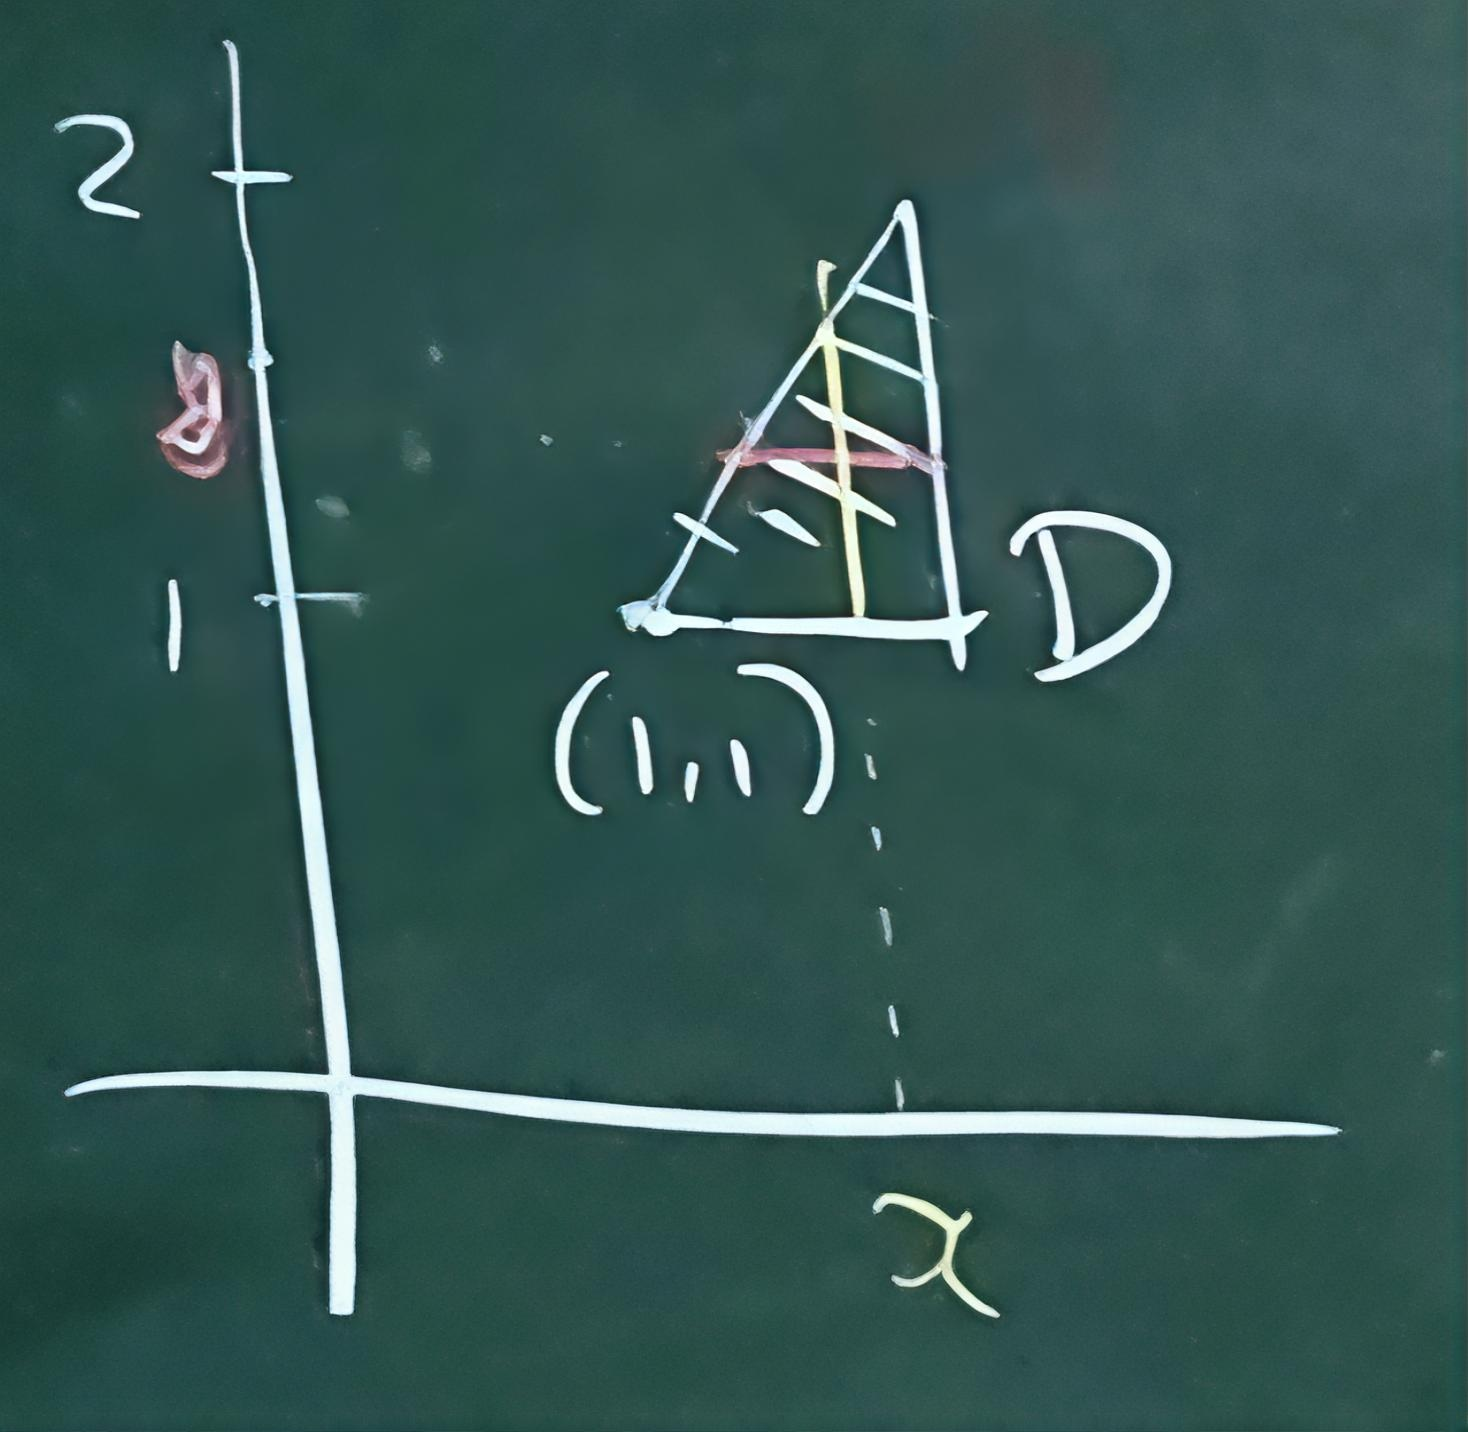
\includegraphics[height=2cm]{chapters/10/01/0306}}\quad
        \begin{matrix}
            \int_1^2y\,\mathrm{d}y\int_y^2\frac{\sin x}{x^2-1}\,\mathrm{d}x & \overset{?}{=} & \int_1^2\,\mathrm{d}x\int_1^x\frac{\sin x}{x^2-1}\cdot y\,\mathrm{d}y                        \\
            \Updownarrow                                                    & =              & \int_1^2\,\mathrm{d}x\left(\frac{\sin x}{x^2-1}\cdot\frac{y^2}{2}\middle|_{y=1}^{y=x}\right) \\
            \iint_Dy\frac{\sin x}{x^2-1}\,\mathrm{d}x\mathrm{d}y            & =              & \int_1^2\frac{1}{2}\sin x\,\mathrm{d}x=\frac{1}{2}(\cos 1-\cos 2)
        \end{matrix}$$

    $y=1$, $\int_1^2\frac{\sin x}{x^2-1}\,\mathrm{d}x$ is an improper integral, and diverges to $+\infty$.

    $y\in(1,2]$, $\int_y^2\frac{\sin x}{x^2-1}\,\mathrm{d}x=\varphi(y)$ all well-defined integral.

    $\varphi(y)$ is continuous (differentiable) on $(1,2]$, but $\lim_{y\to1^+}\varphi(y)=+\infty$, then
    $$\raisebox{-0.5\height}{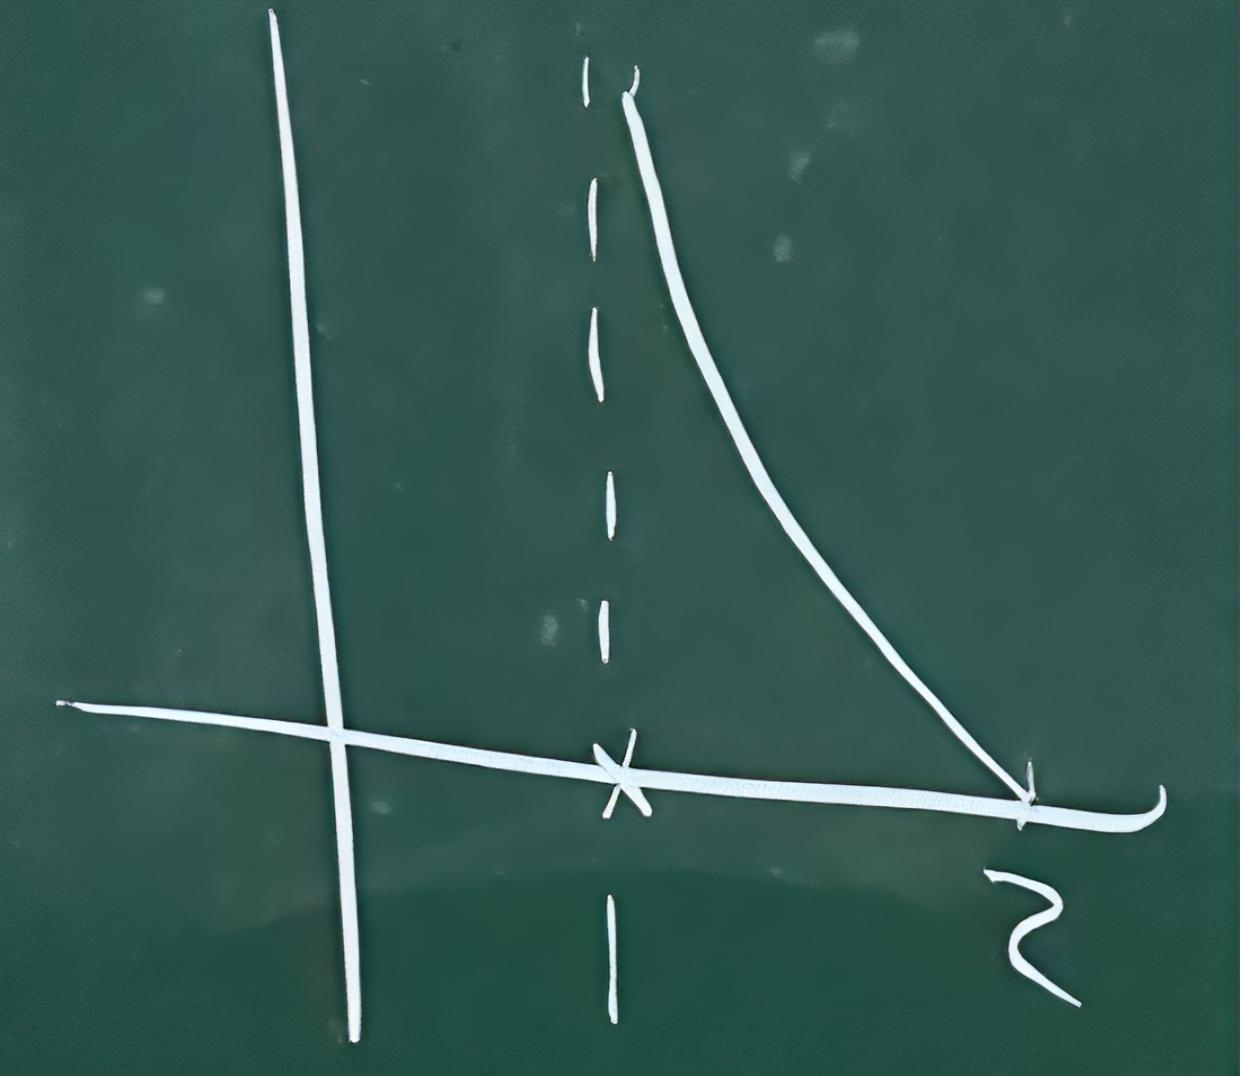
\includegraphics[height=1.5cm]{chapters/10/01/0307}}\quad\int_1^2y\,\mathrm{d}y\int_y^2\frac{\sin x}{x^2-1}\,\mathrm{d}x=\int_1^2y\cdot\varphi(y)\,\mathrm{d}y$$
    is an improper integral on $[1,2]$.

    \begin{align*}
        \raisebox{-0.5\height}{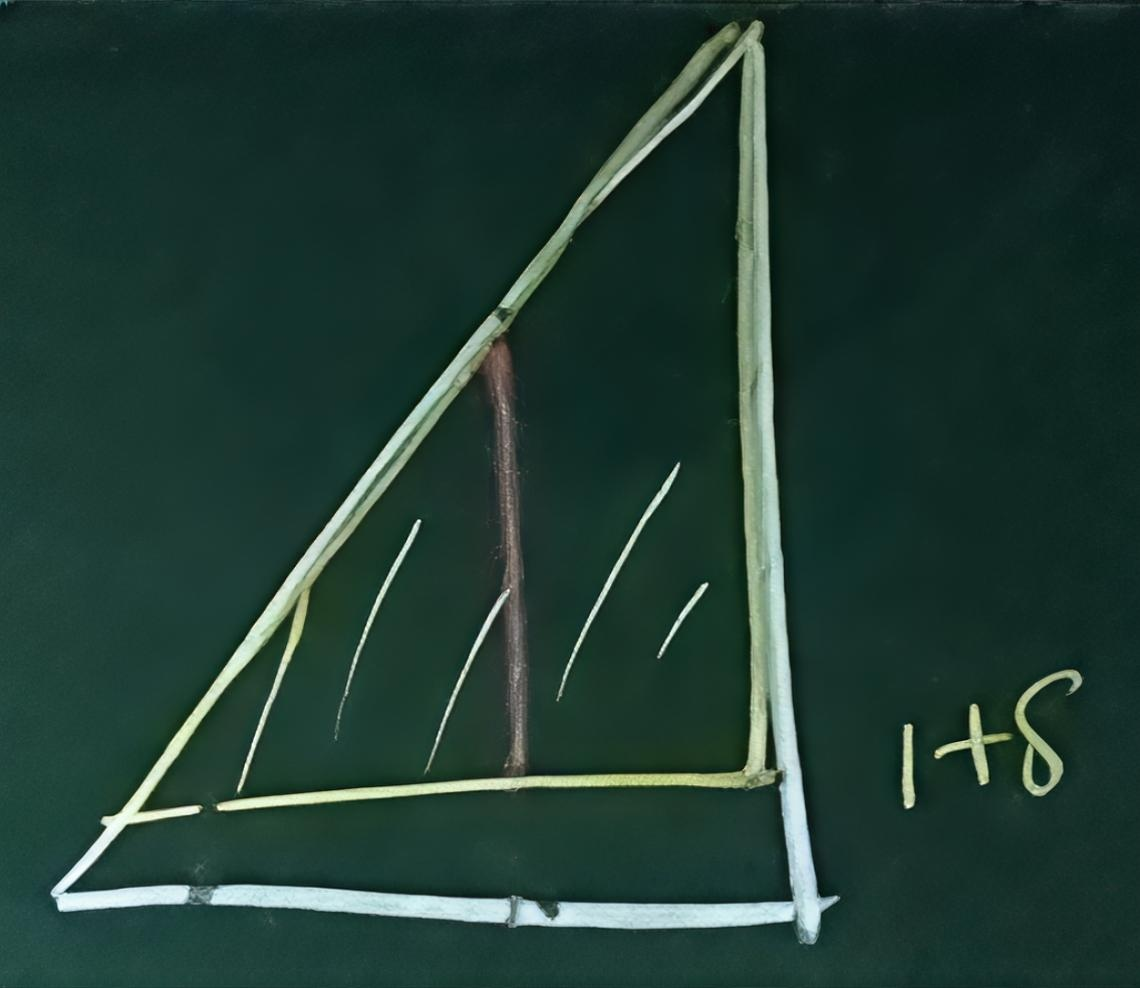
\includegraphics[height=2cm]{chapters/10/01/0308}}\quad
        \int_1^2y\varphi(y)\,\mathrm{d}y
         & =\lim_{\delta\to0^+}\boxed{\int_{1+\delta}^2y\,\mathrm{d}y\int_y^2\frac{\sin x}{x^2-1}\,\mathrm{d}x}                             \\
         & =\lim_{\delta\to0^+}\int_{1+\delta}^2\,\mathrm{d}x\int_{1+\delta}^{x}\frac{\sin x}{x^2-1}\cdot y\,\mathrm{d}y                    \\
         & =\lim_{\delta\to0^+}\frac{1}{2}\int_{1+\delta}^2\frac{\sin x}{x^2-1}\left(x^2-(1+\delta^2)\right)\,\mathrm{d}x                   \\
         & =\lim_{\delta\to0^+}\frac{1}{2}\int_{1+\delta}^2\left(\sin x-\left(2\delta+\delta^2\right)\frac{\sin x}{x^2-1}\right)\mathrm{d}x
    \end{align*}

    $$\left|-\frac{2\delta+\delta^2}{2}\int_{1+\delta}^2\frac{\sin x}{x^2-1}\,\mathrm{d}x\right|\leq\frac{2\delta+\delta^2}{2}\int_{1+\delta}^2\frac{1}{(x-1)^2}\,\mathrm{d}x=\frac{2\delta+\delta^2}{4}\boxed{\log\frac{1}{\delta}}\to0\quad\text{(as $\delta\to0$)}$$

    $$\frac{\int_2^{1+\delta}\frac{\sin x}{x^2-1}\,\mathrm{d}x}{\frac{1}{2\delta+\delta^2}}\frac{\frac{\sin(1+\delta)}{(1+\delta)^2-1}}{-\frac{2}{(2\delta+\delta^2)^2}}=\frac{\sin(1+\delta)}{2\delta+\delta^2}(2\delta+\delta^2)^2\to0$$
\end{example}

